% Intended LaTeX compiler: pdflatex
\documentclass[11pt]{article}
\usepackage[utf8]{inputenc}
\usepackage[T1]{fontenc}
\usepackage{graphicx}
\usepackage{grffile}
\usepackage{longtable}
\usepackage{wrapfig}
\usepackage{rotating}
\usepackage[normalem]{ulem}
\usepackage{amsmath}
\usepackage{textcomp}
\usepackage{amssymb}
\usepackage{capt-of}
\usepackage{hyperref}
\documentclass{article}
\addtolength{\voffset}{-2.25cm}
\usepackage[document]{ragged2e}
\usepackage{fancyhdr}
\pagestyle{fancy}
\fancyhf{}
\lhead{Minor scales and modes for ii-v-i progressions}
\rhead{Bartev - 2020-12-28}
\cfoot{\thepage}
\author{Bartev Vartanian}
\date{2020-12-28}
\title{Minor scales and modes for ii-v-i progressions}
\hypersetup{
 pdfauthor={Bartev Vartanian},
 pdftitle={Minor scales and modes for ii-v-i progressions},
 pdfkeywords={},
 pdfsubject={},
 pdfcreator={Emacs 27.1 (Org mode 9.3)}, 
 pdflang={English}}
\begin{document}

\maketitle

\section*{Comments}
\label{sec:org271aaef}

These are some scales from the 12-2020 Chad lesson.

\section*{Major scale}
\label{sec:org7ca44aa}

The C major scale (Ionian mode)

\begin{center}
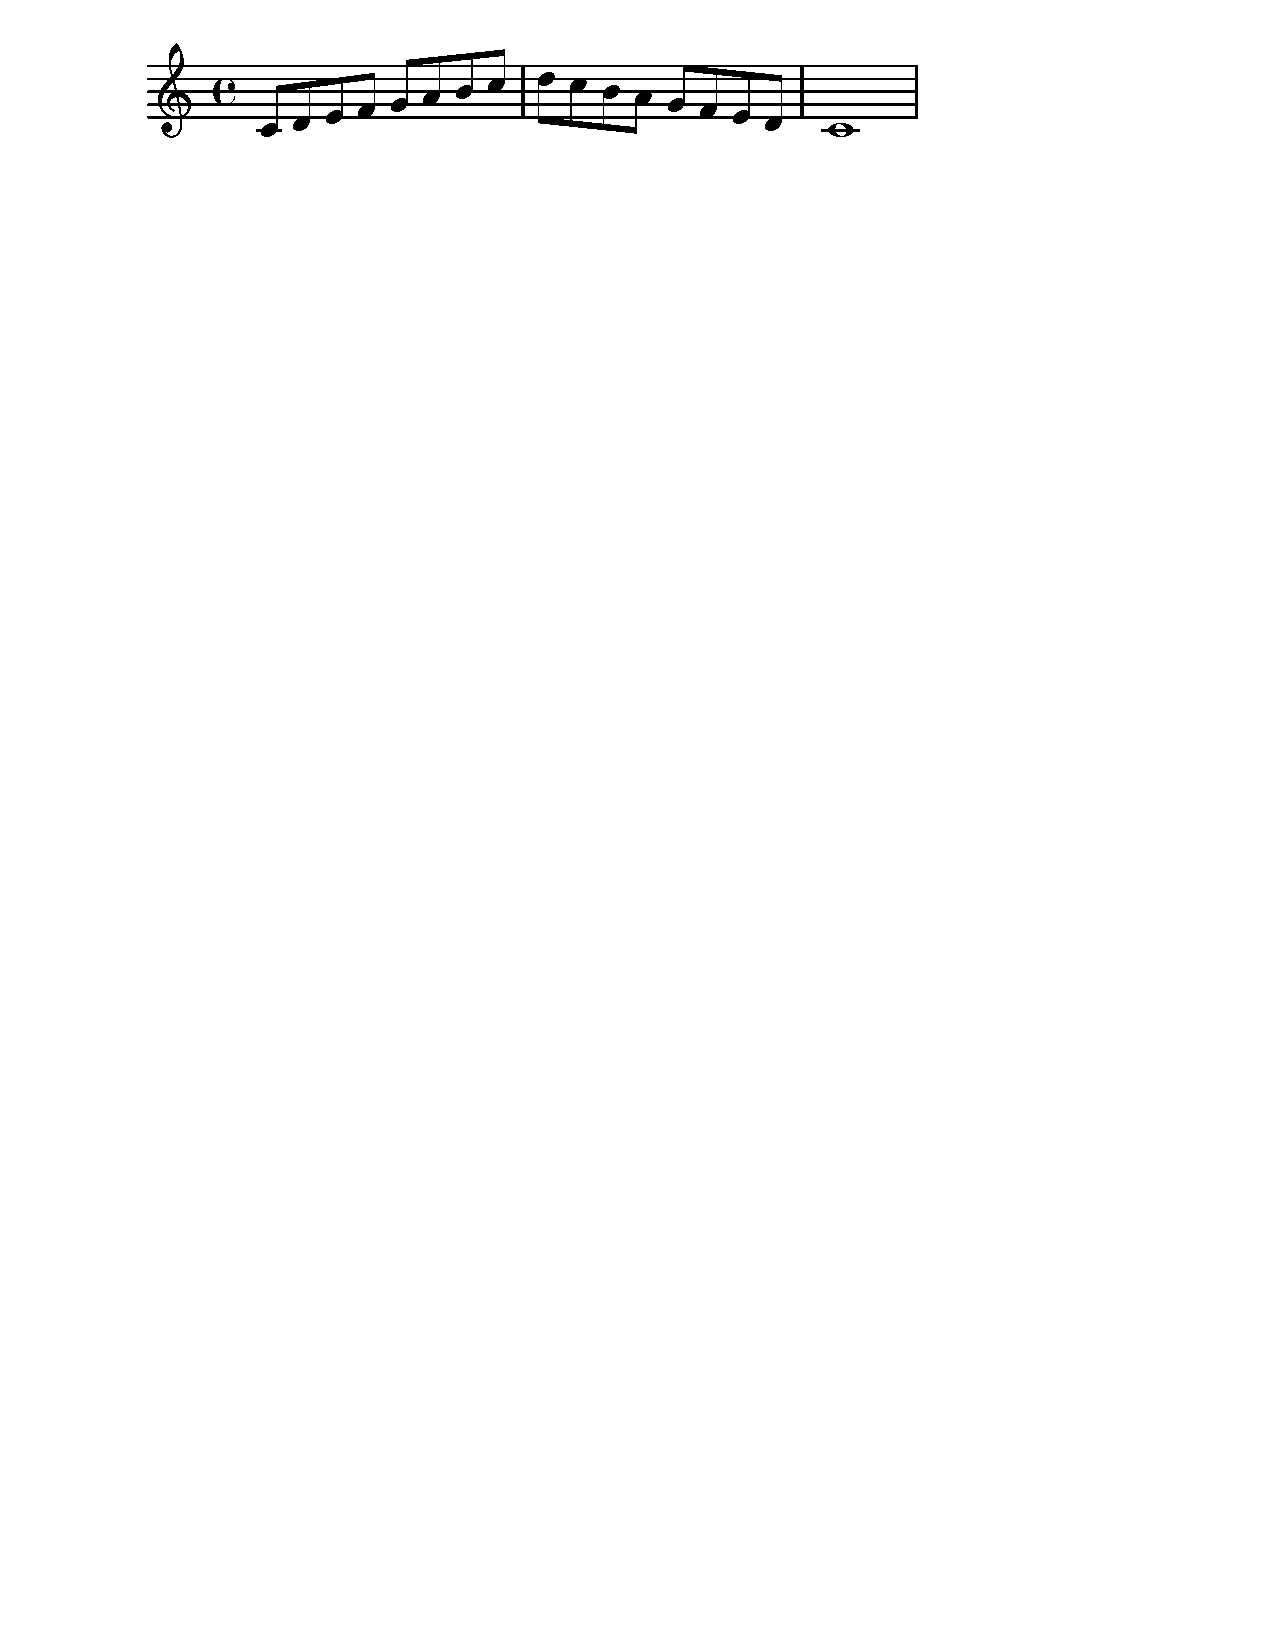
\includegraphics[width=.9\linewidth]{c_major.pdf}
\end{center}

\section*{Natural minor scale (Aeolian mode)}
\label{sec:orgf11dfcb}


The A natural minor is built off the 6th degree of its relative major (C).

It has a \(\flat{3}\), \(\flat{6}\)  and \(\flat{7}\)  relative to the A major scale.

\begin{center}
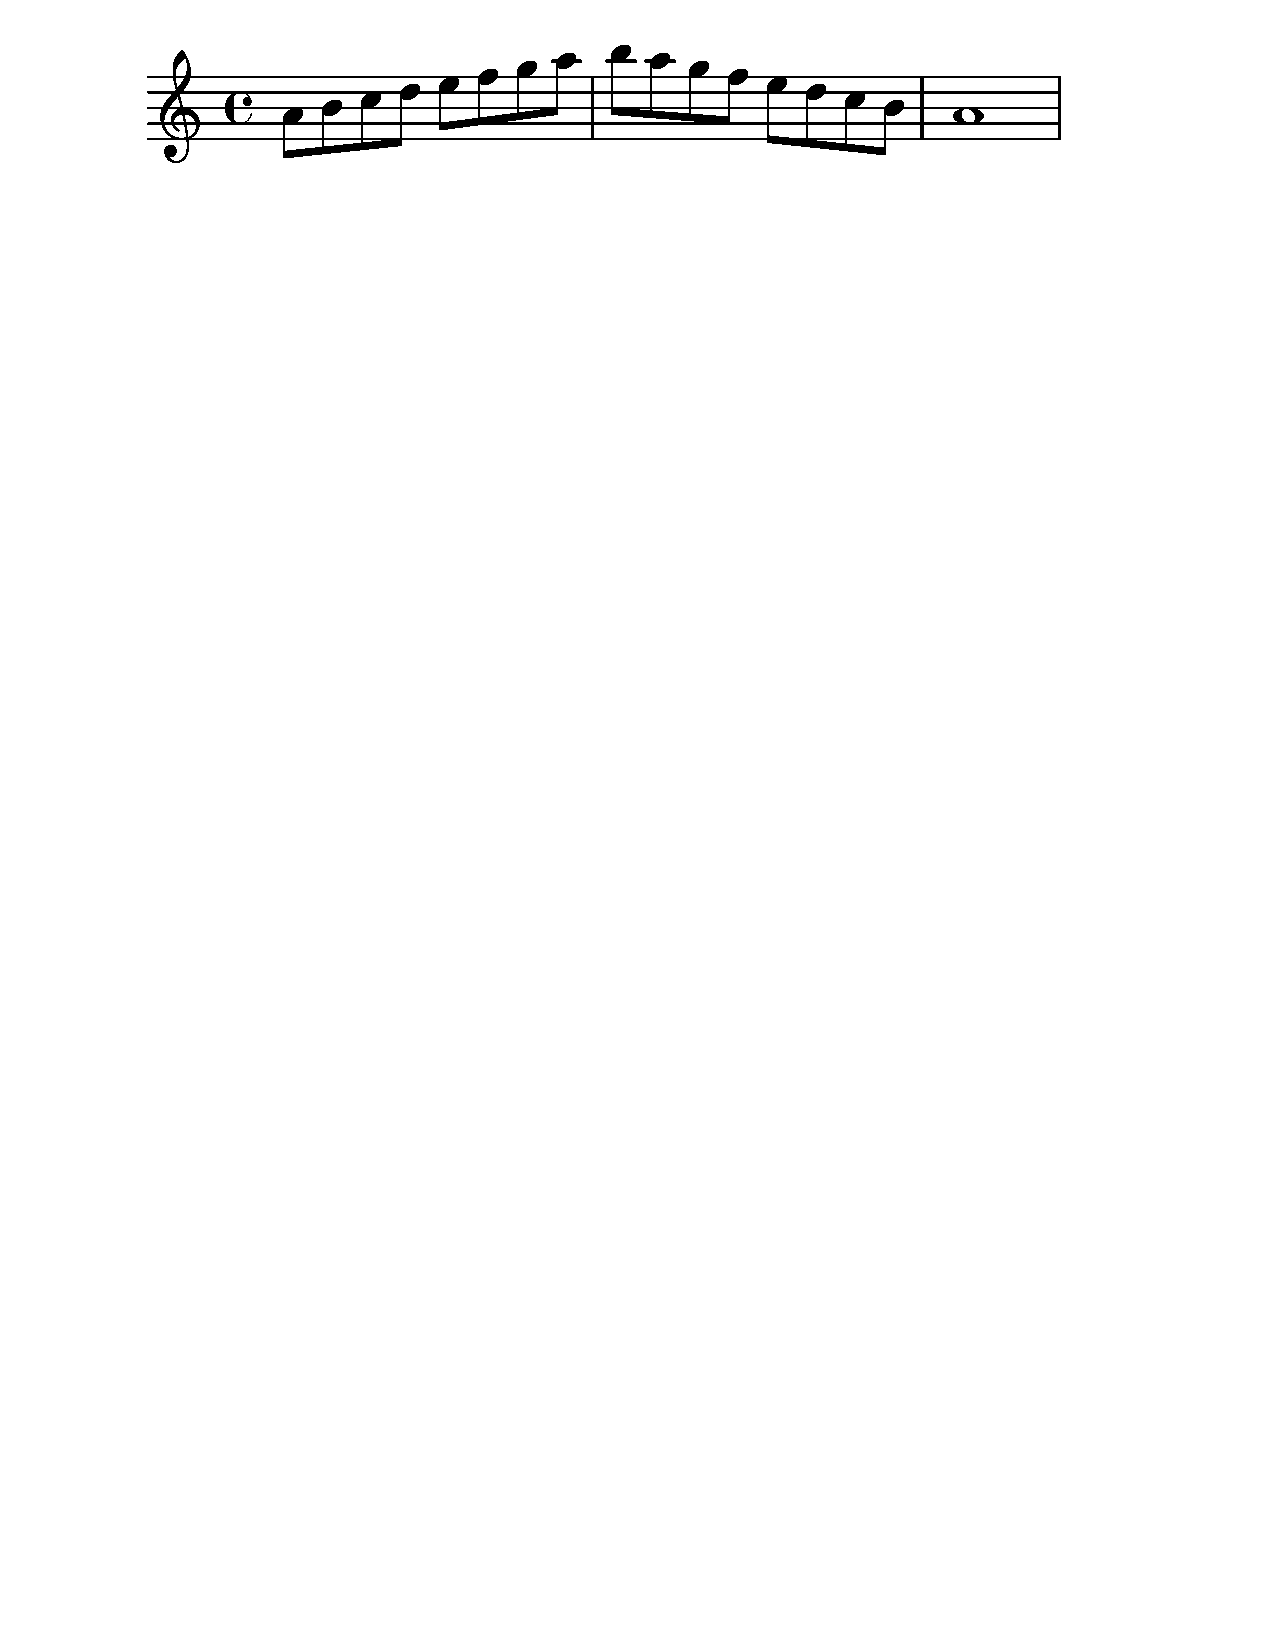
\includegraphics[width=.9\linewidth]{a_natural_minor.pdf}
\end{center}

\section*{Harmonic minor scale (Aeolian \(\sharp{7}\))}
\label{sec:orge4d675c}

The A harmonic minor is built off the 6th degree of its relative major (C).

Relative to the A major scale, it has a \(\flat{3}\) and \(\flat{6}\).

Relative to the A natural minor scale, it has a \(\sharp{7}\).

\begin{center}
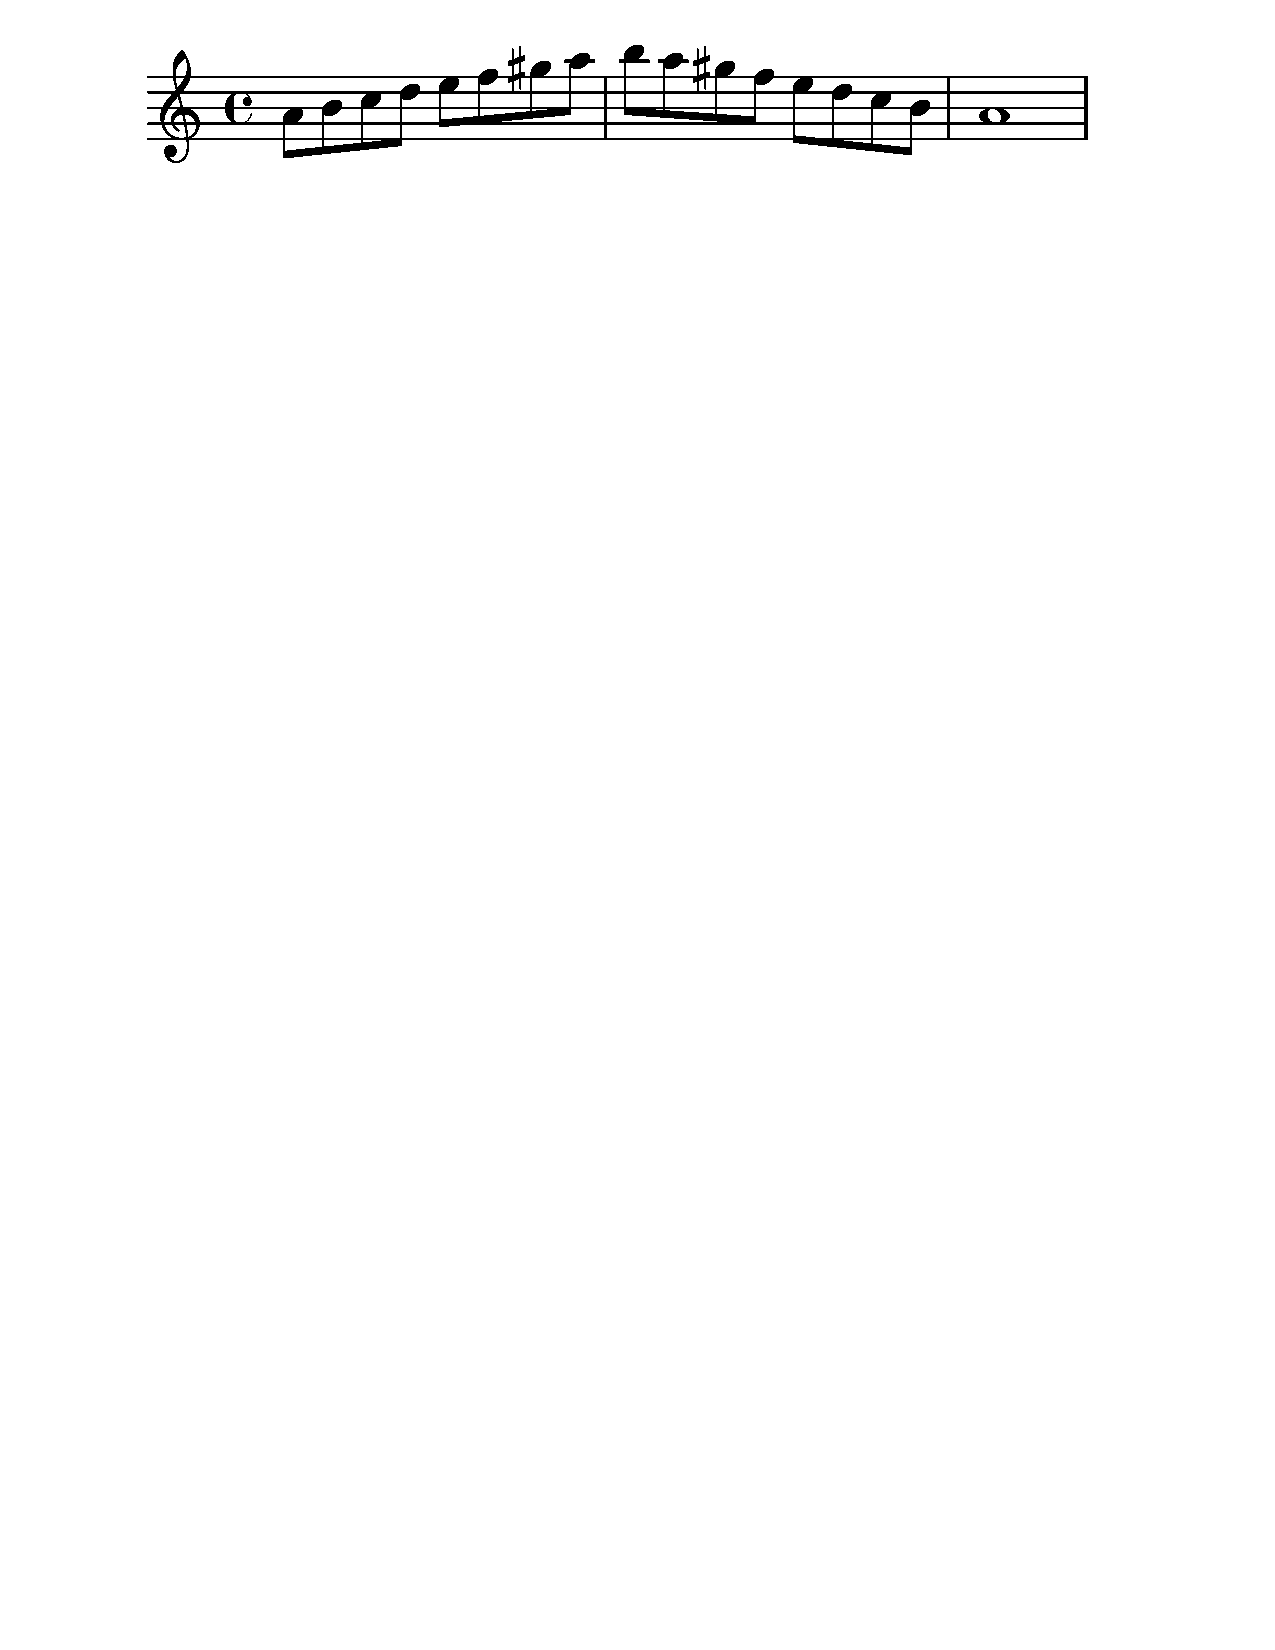
\includegraphics[width=.9\linewidth]{a_harmonic_minor.pdf}
\end{center}

\section*{Melodic minor scale}
\label{sec:orgb64b729}

The A melodic minor is built off the 6th degree of its relative major (C).
On the way up, it has a \(\flat{3}\) relative to the major key, but on the way down it is the same as the natural minor.

Relative to the A major scale, it has a \(\flat{3}\) while ascending, and a \(\flat{3}\), \(\flat{6}\)  and \(\flat{7}\) while descending

Relative to the A natural minor scale, it has a \(\sharp{6}\) and \(\sharp{7}\) while ascending only.

\begin{center}
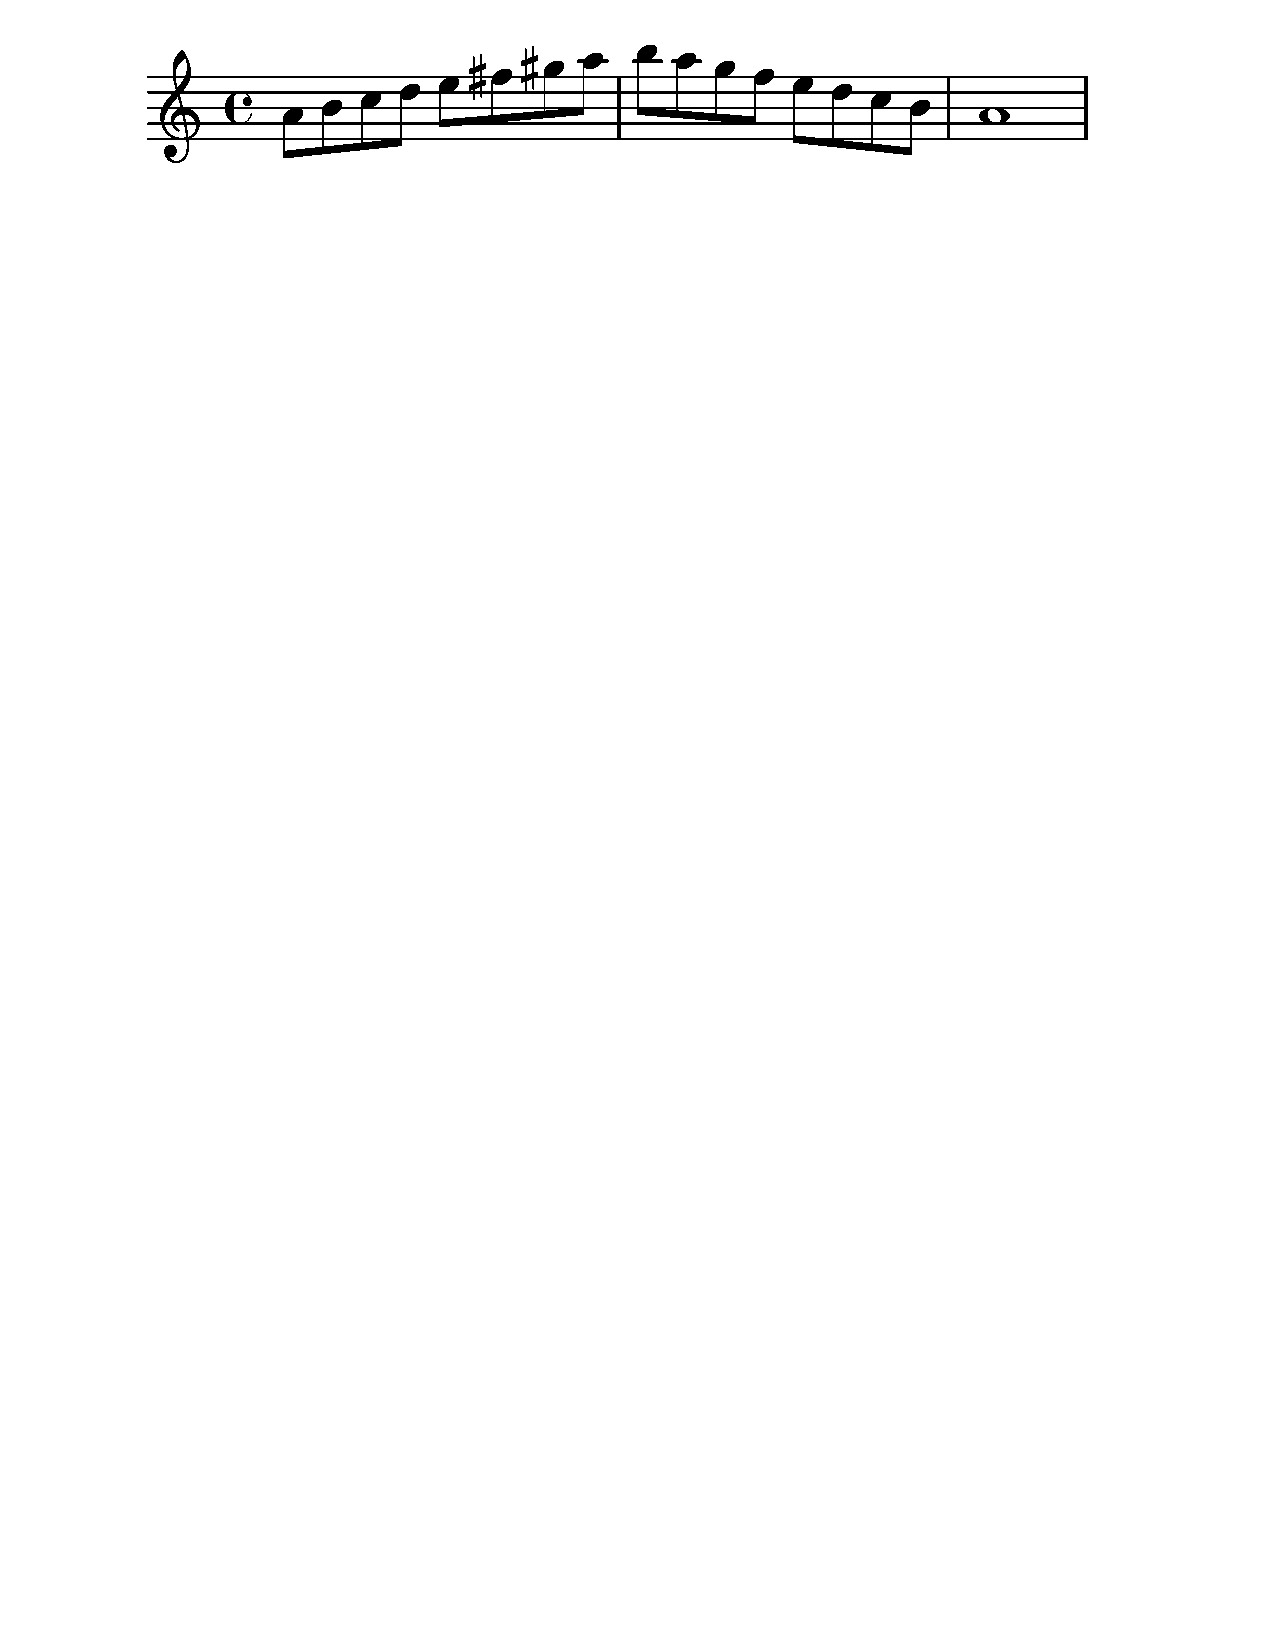
\includegraphics[width=.9\linewidth]{a_melodic_minor.pdf}
\end{center}

\section*{Phrygian mode (natural minor + \(\flat{2}\))}
\label{sec:org109a76a}

The Phrygian mode essentially adds 4 flats.

Relative to the major key, it has a \(\flat{2}\), \(\flat{3}\), \(\flat{6}\)  and \(\flat{7}\).

Relative to the natural minor, it has a \(\flat{2}\).

\subsection*{Chords}
\label{sec:org0ad0a48}

Use with a sus\(4\flat{9}\)

\begin{center}
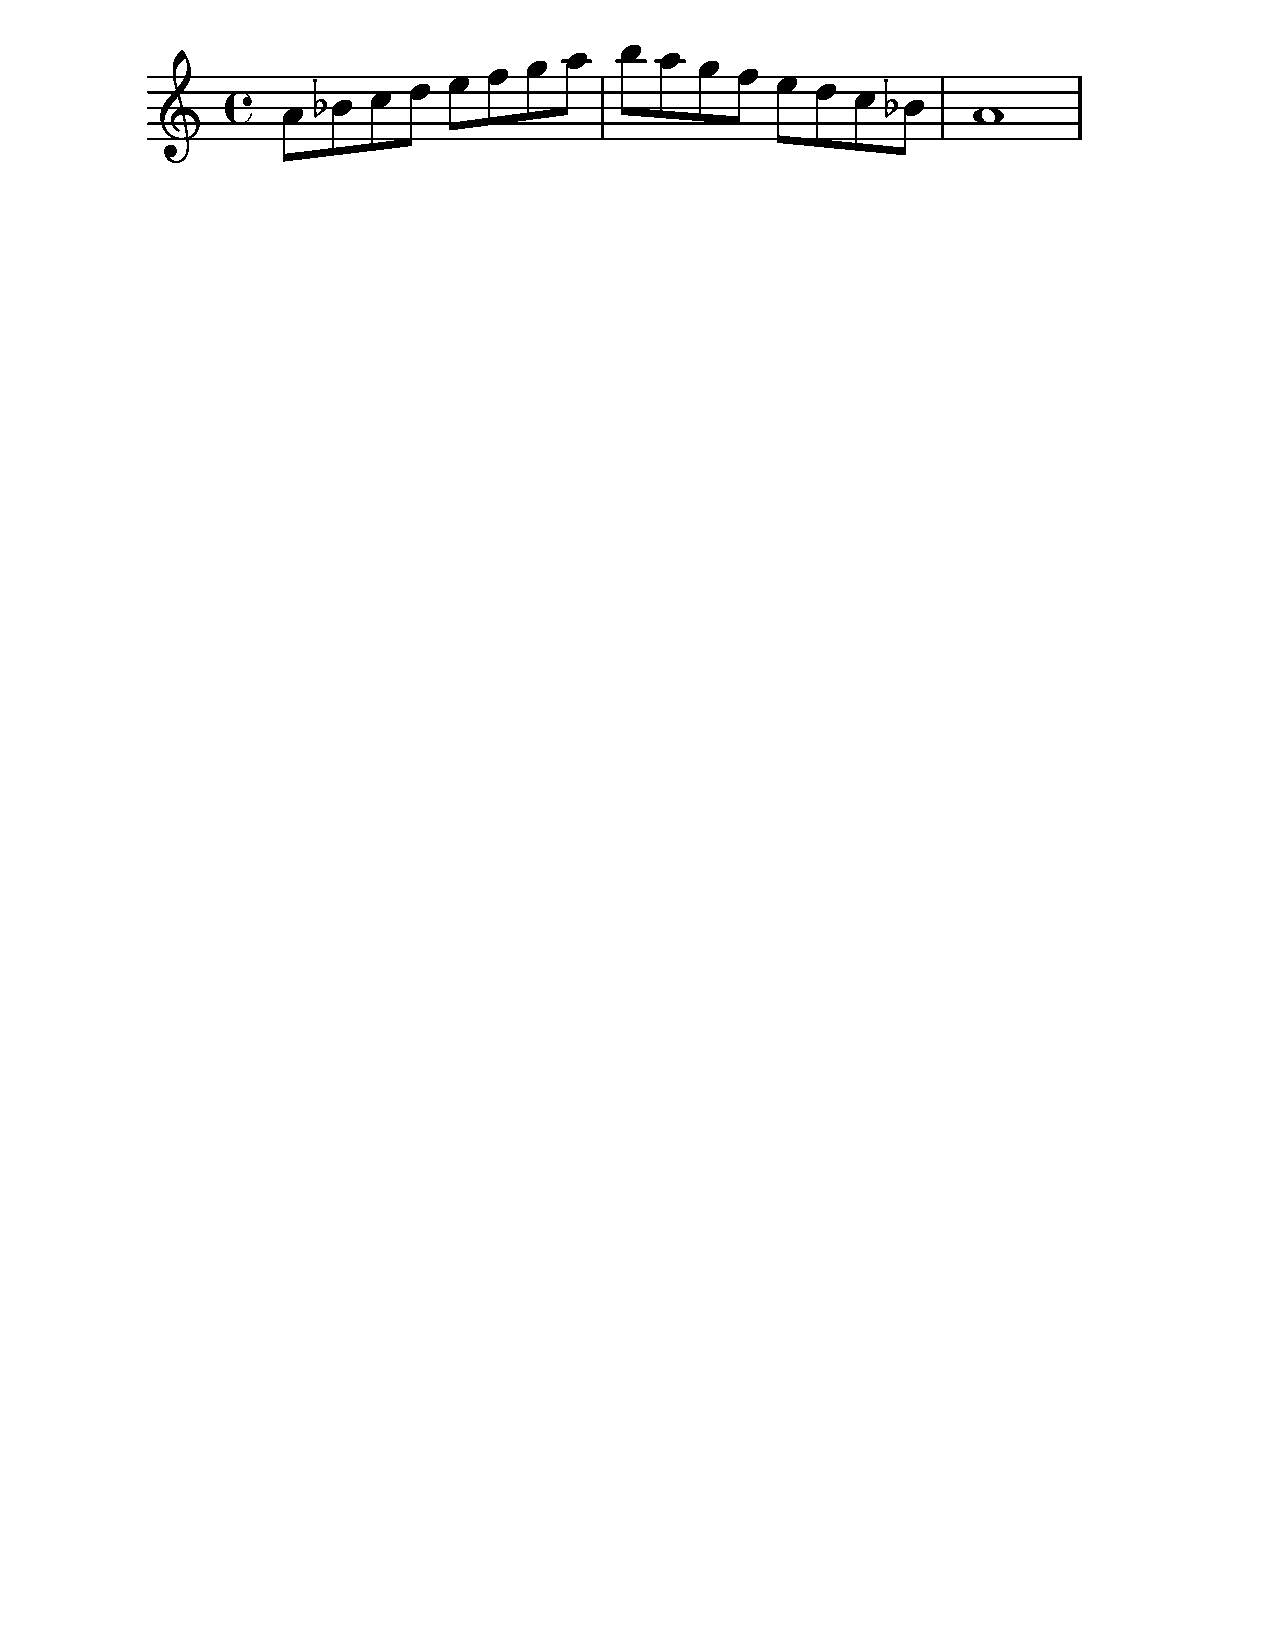
\includegraphics[width=.9\linewidth]{a_phrygian_mode.pdf}
\end{center}

\section*{Phrygian dominant (aka Spanish gypsy scale)}
\label{sec:org980f80a}

The Phrygian dominant has a \(\sharp{3}\) relative to the Phrygian mode

Relative to the major key, it has a \(\flat{2}\), \(\flat{6}\)  and \(\flat{7}\).

Relative to the natural minor, it has a \(\flat{2}\) and \(\sharp{3}\).


\begin{center}
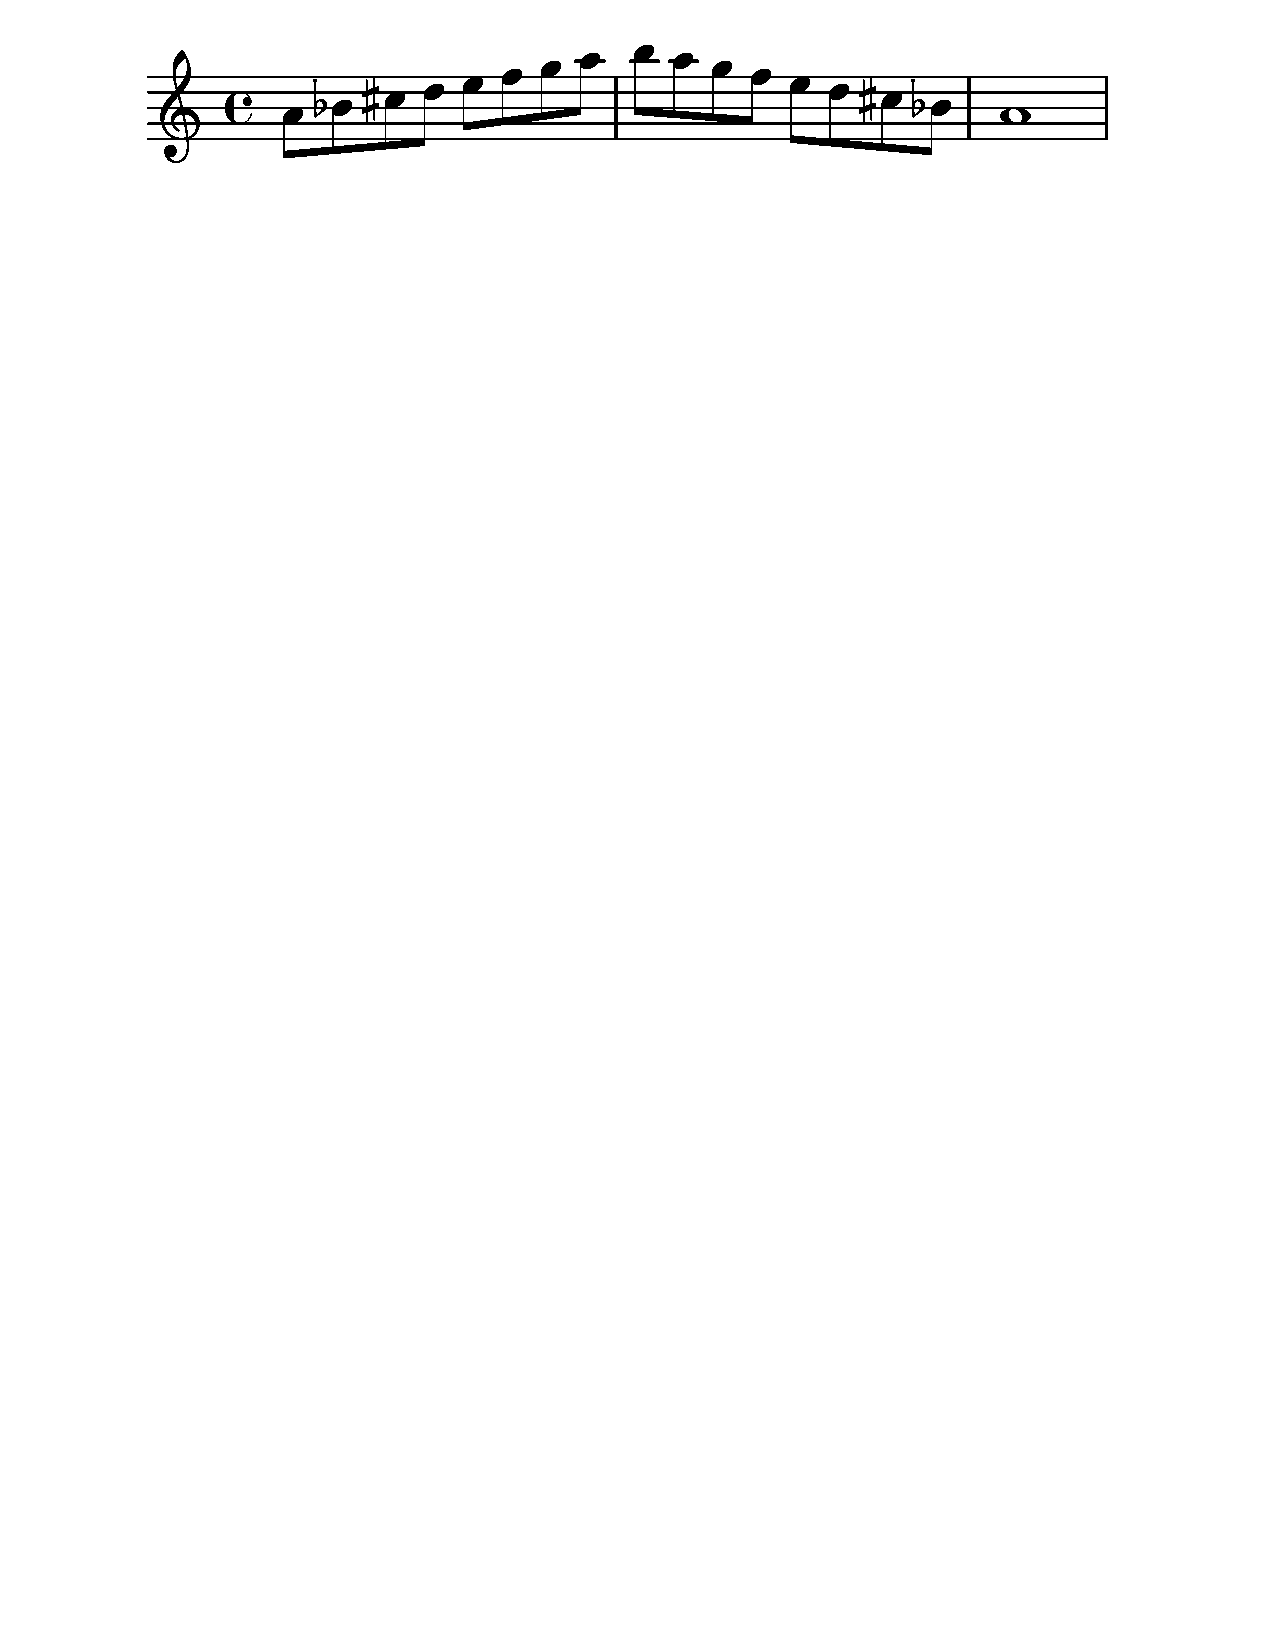
\includegraphics[width=.9\linewidth]{a_phrygian_dominant.pdf}
\end{center}

\section*{Locrian}
\label{sec:org341fd75}

The Locrian mode has 5 flats relative to the major scale.

It has a key signature of a 1/2 step up.

Relative to the major key, it has a \(\flat{2}\), \(\flat{3}\), \(\flat{5}\), \(\flat{6}\)  and \(\flat{7}\).

Relative to the natural minor, it has a \(\flat{2}\) and \(\flat{5}\).


\begin{center}
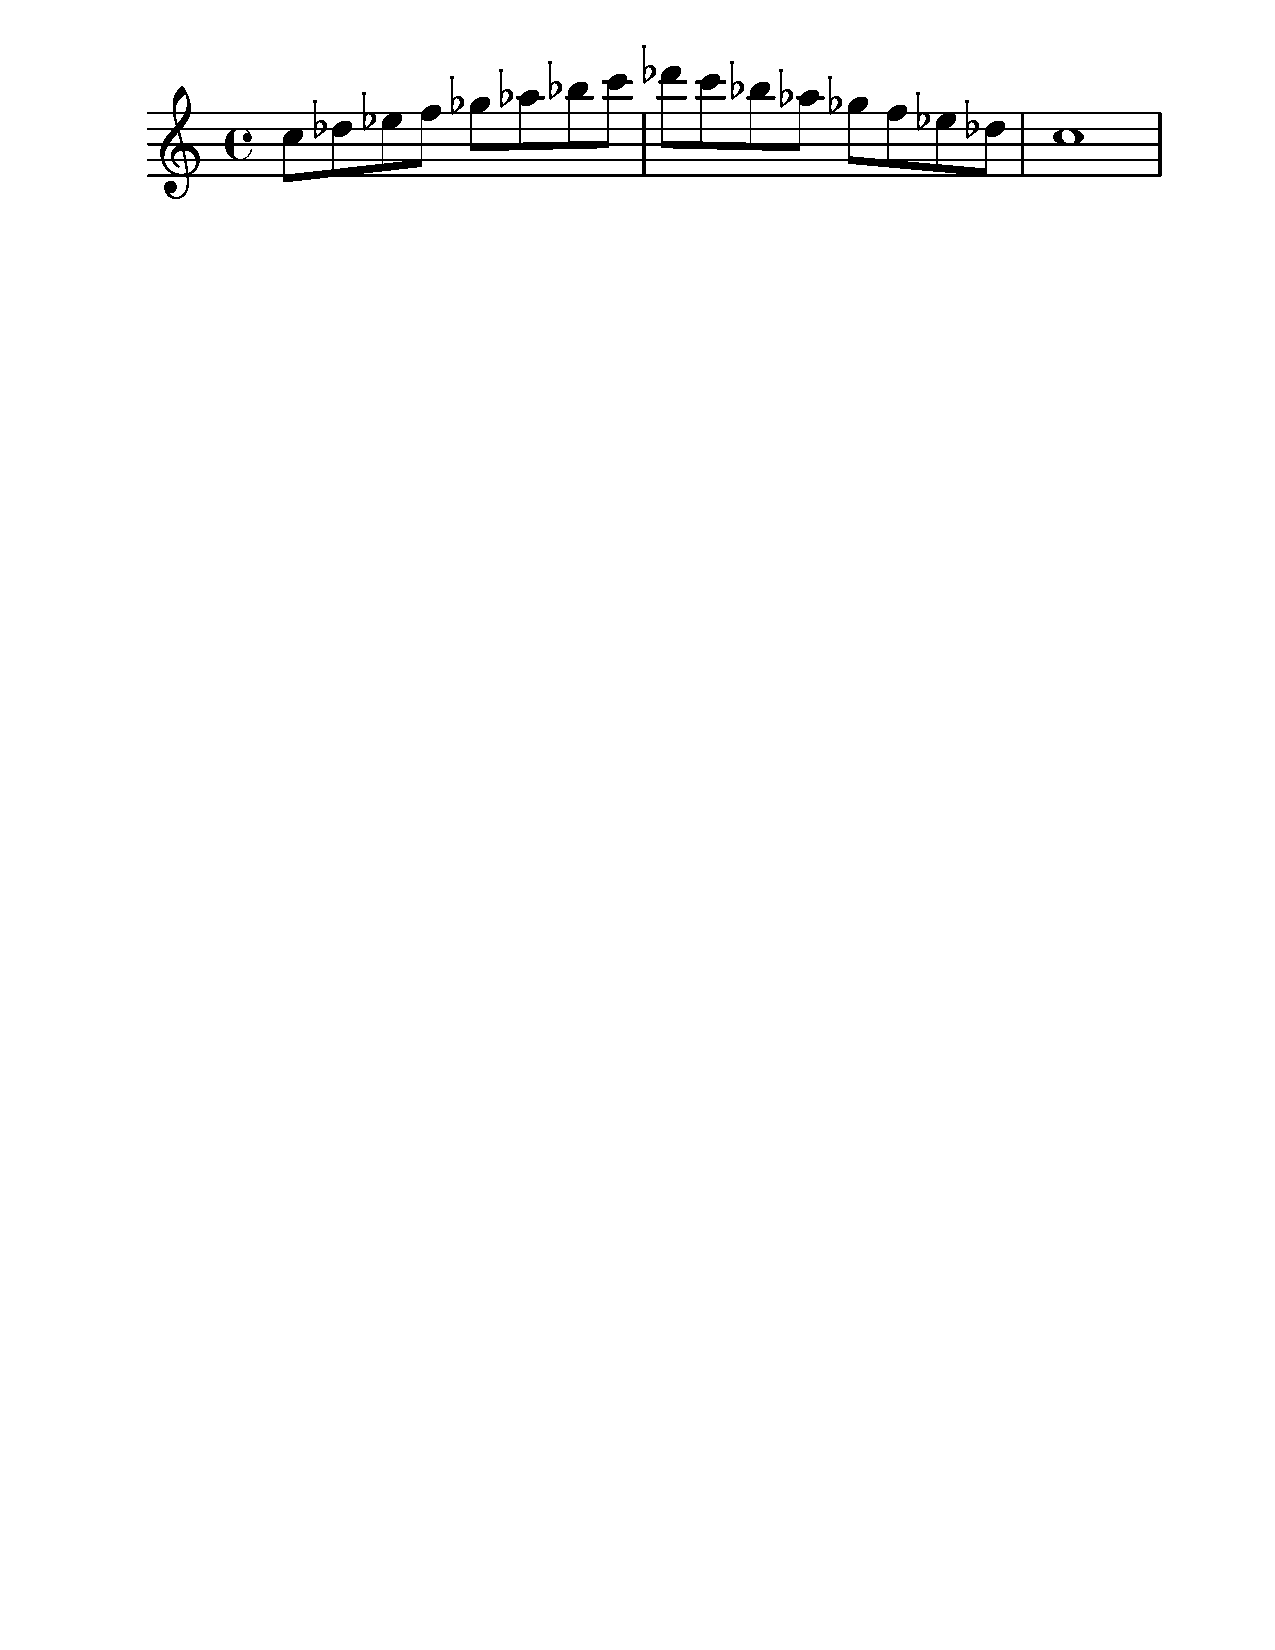
\includegraphics[width=.9\linewidth]{c_locrian.pdf}
\end{center}

\section*{Locrian nat 2}
\label{sec:orgce24e4d}

The Locrian nat 2 scale is similar to the Locrian mode, but with a raised 2nd.

Relative to the Locrian mode, it has a \(\sharp{2}\).


\begin{center}
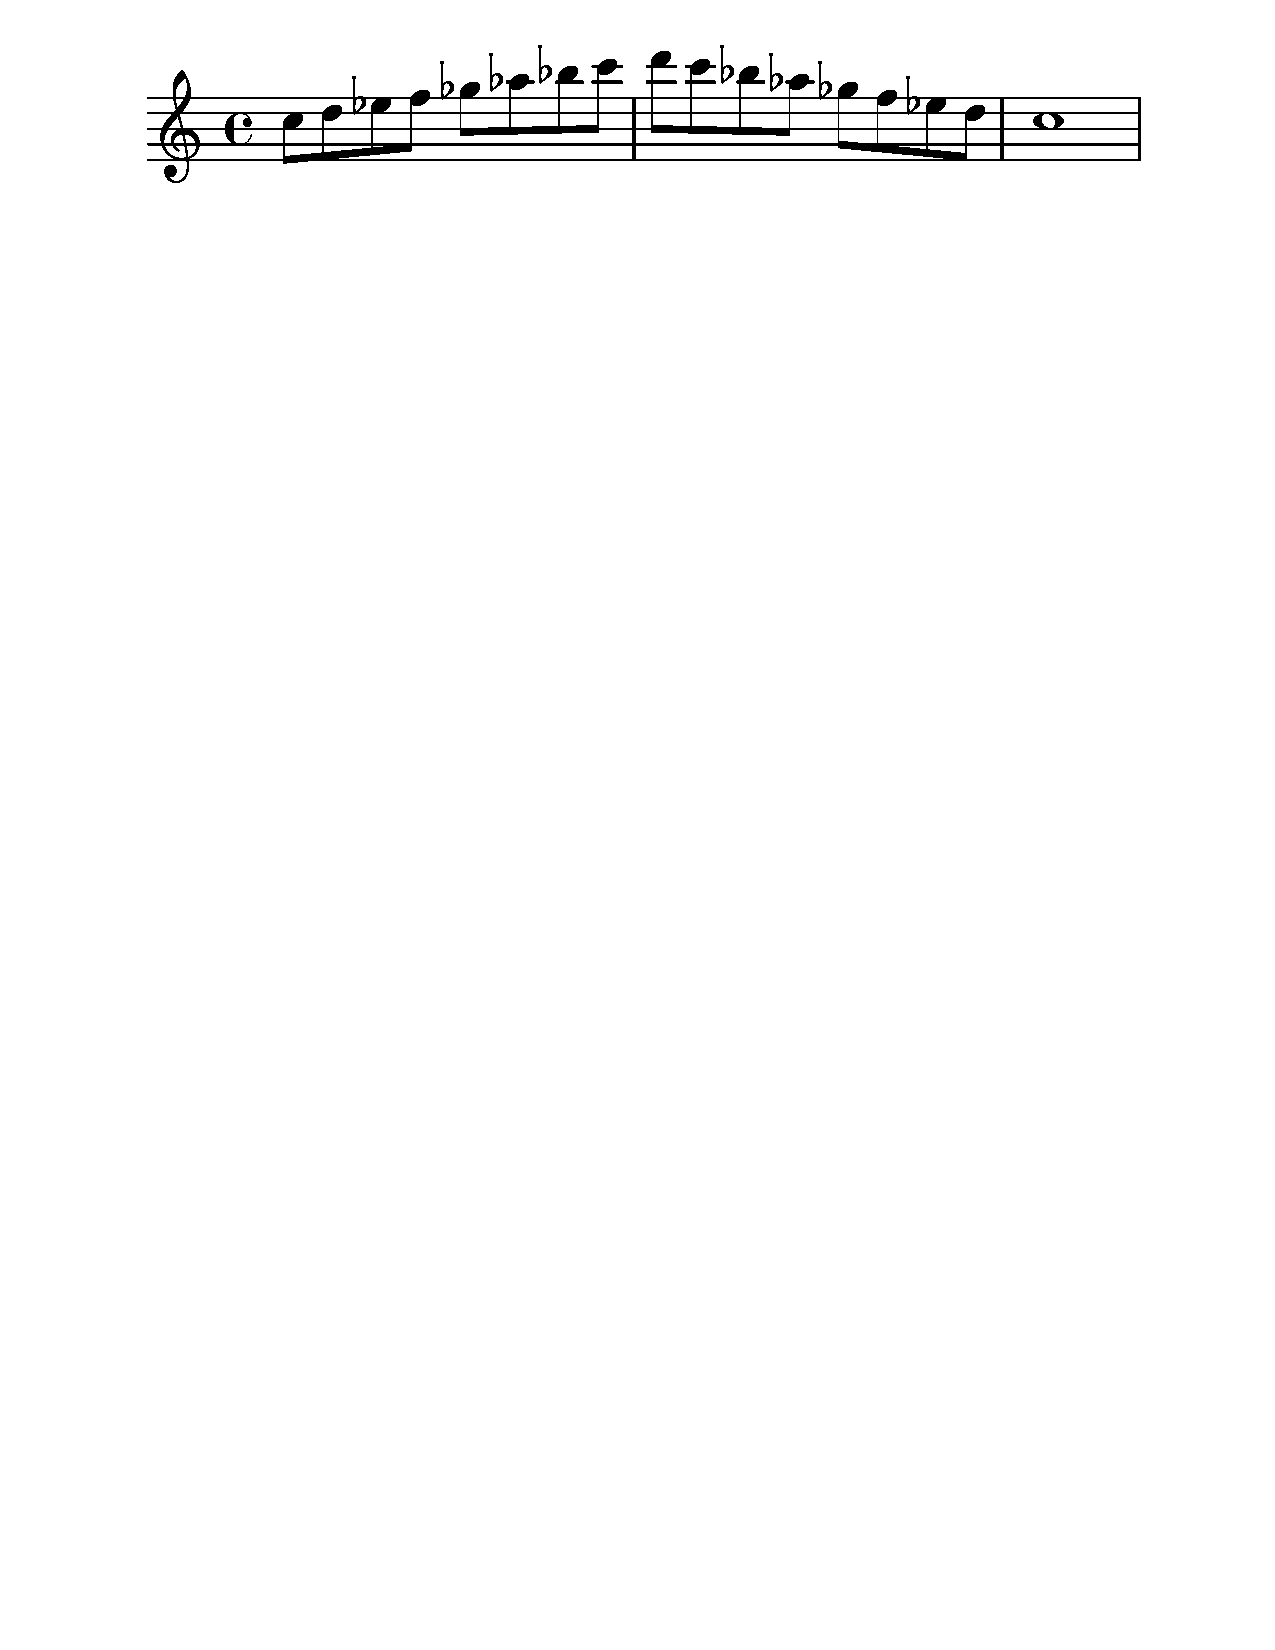
\includegraphics[width=.9\linewidth]{c_locrian_nat_2.pdf}
\end{center}
\end{document}
